\documentclass[]{book}
\usepackage{lmodern}
\usepackage{amssymb,amsmath}
\usepackage{ifxetex,ifluatex}
\usepackage{fixltx2e} % provides \textsubscript
\ifnum 0\ifxetex 1\fi\ifluatex 1\fi=0 % if pdftex
  \usepackage[T1]{fontenc}
  \usepackage[utf8]{inputenc}
\else % if luatex or xelatex
  \ifxetex
    \usepackage{mathspec}
  \else
    \usepackage{fontspec}
  \fi
  \defaultfontfeatures{Ligatures=TeX,Scale=MatchLowercase}
\fi
% use upquote if available, for straight quotes in verbatim environments
\IfFileExists{upquote.sty}{\usepackage{upquote}}{}
% use microtype if available
\IfFileExists{microtype.sty}{%
\usepackage{microtype}
\UseMicrotypeSet[protrusion]{basicmath} % disable protrusion for tt fonts
}{}
\usepackage[margin=1in]{geometry}
\usepackage{hyperref}
\hypersetup{unicode=true,
            pdftitle={Crime Mapping and Spatial Analysis},
            pdfauthor={John Palmer},
            pdfborder={0 0 0},
            breaklinks=true}
\urlstyle{same}  % don't use monospace font for urls
\usepackage{natbib}
\bibliographystyle{apalike}
\usepackage{longtable,booktabs}
\usepackage{graphicx,grffile}
\makeatletter
\def\maxwidth{\ifdim\Gin@nat@width>\linewidth\linewidth\else\Gin@nat@width\fi}
\def\maxheight{\ifdim\Gin@nat@height>\textheight\textheight\else\Gin@nat@height\fi}
\makeatother
% Scale images if necessary, so that they will not overflow the page
% margins by default, and it is still possible to overwrite the defaults
% using explicit options in \includegraphics[width, height, ...]{}
\setkeys{Gin}{width=\maxwidth,height=\maxheight,keepaspectratio}
\IfFileExists{parskip.sty}{%
\usepackage{parskip}
}{% else
\setlength{\parindent}{0pt}
\setlength{\parskip}{6pt plus 2pt minus 1pt}
}
\setlength{\emergencystretch}{3em}  % prevent overfull lines
\providecommand{\tightlist}{%
  \setlength{\itemsep}{0pt}\setlength{\parskip}{0pt}}
\setcounter{secnumdepth}{5}
% Redefines (sub)paragraphs to behave more like sections
\ifx\paragraph\undefined\else
\let\oldparagraph\paragraph
\renewcommand{\paragraph}[1]{\oldparagraph{#1}\mbox{}}
\fi
\ifx\subparagraph\undefined\else
\let\oldsubparagraph\subparagraph
\renewcommand{\subparagraph}[1]{\oldsubparagraph{#1}\mbox{}}
\fi

%%% Use protect on footnotes to avoid problems with footnotes in titles
\let\rmarkdownfootnote\footnote%
\def\footnote{\protect\rmarkdownfootnote}

%%% Change title format to be more compact
\usepackage{titling}

% Create subtitle command for use in maketitle
\providecommand{\subtitle}[1]{
  \posttitle{
    \begin{center}\large#1\end{center}
    }
}

\setlength{\droptitle}{-2em}

  \title{Crime Mapping and Spatial Analysis}
    \pretitle{\vspace{\droptitle}\centering\huge}
  \posttitle{\par}
  \subtitle{Lab Manual}
  \author{John Palmer}
    \preauthor{\centering\large\emph}
  \postauthor{\par}
      \predate{\centering\large\emph}
  \postdate{\par}
    \date{2020-02-06}

\usepackage{booktabs}

\begin{document}
\maketitle

{
\setcounter{tocdepth}{1}
\tableofcontents
}
\hypertarget{cover}{%
\chapter*{Cover}\label{cover}}
\addcontentsline{toc}{chapter}{Cover}

\hypertarget{introduction}{%
\chapter*{Introduction}\label{introduction}}
\addcontentsline{toc}{chapter}{Introduction}

This manual is intended to function as a companion to the \emph{Crime Mapping and Spatial Analysis} labs as well as a stand-along reference for working with QGIS, Stata, and R for mapping and analysis. Each chapter walks you through a particular task or set of tasks, usually with an exercise to serve as an example. These are organized according to the class lab sessions but can also be followed intependently or used as a reference.

\hypertarget{accessing-qgis}{%
\section*{Accessing QGIS}\label{accessing-qgis}}
\addcontentsline{toc}{section}{Accessing QGIS}

QGIS is free and open source software, which you can download from \url{https://qgis.org}. At the time of writing, version 3.4 is the most recent long-term stable release and this manual is based on that version. When installing QGIS, leaving all of the default options as they are should be fine for purposes of this manual. The Windows installation includes a number of different choices for running QGIS; you shoud simply select the normal desktop version.

\hypertarget{accessing-stata}{%
\section*{Accessing Stata}\label{accessing-stata}}
\addcontentsline{toc}{section}{Accessing Stata}

Stata is proprietary software, which cannot be freely downloaded if have not purchased a license. However, as a UPF student, you have free access to Stata on the UPF lab computers and through UPF's \emph{MyApps} platform. The latter requires an internet connection and has some limitations in terms of resources, but you can access it from outside UPF using your own computer and a web browser.

To access Stata through \emph{MyApps}, open a web browser and go to \url{https://myapps.upf.edu}. Log in using your UPF user ID (uxxxxx) and the password you use for logging into UPF computers (i.e.~your birthdate, written as DDMMYYYY). Remember that this is not necessarily the password you use for Campus Global; your browser may have that Campus Global password stored, in which case you will need to manually change it each time. On the login page, you will need to choose between using \emph{vWorkspace Connector} or simply through your web browser with HTML5. The first option allows you to access local files on your computer, but it can be slow and ``buggy'', particularly on Macs. To follow this approach, click the \emph{Install} button on the page you reach after logging in. The second option can be faster, but any files you want to use will need to be first uploaded through the UPF MyCloud. To follow this approach, click the \emph{Continue} button on the page after login, and then flip the \emph{HTML5} switch to the on position at the top right of your screen.

\hypertarget{accessing-r}{%
\section*{Accessing R}\label{accessing-r}}
\addcontentsline{toc}{section}{Accessing R}

R is free and open source software, which you can download from \url{https://cran.r-project.org/}. You will normally want to install the latest release from that site, and to then install a good text editor or Integrated Development Environment (IDE). An excellent choice for the latter is the (free) Open Source Edition of RStudio, which you can download from \url{https://www.rstudio.com}. R and RStudio are also both available on the lab computers. This manual will assume that you are running RStudio.

\hypertarget{lab-instructions}{%
\chapter*{Lab Instructions}\label{lab-instructions}}
\addcontentsline{toc}{chapter}{Lab Instructions}

This section provides instructions for each lab session

\hypertarget{lab-1-9-january-2020}{%
\section*{Lab 1: 9 January 2020}\label{lab-1-9-january-2020}}
\addcontentsline{toc}{section}{Lab 1: 9 January 2020}

The core of criminology research involves observing the world around you, thinking about it, and communicating your thoughts to others. Computers can be useful tools for this, and most of the labs will focus on how to make use of them. Yet, computers can also get in the way. They can distort our observations and encourage us to think and communicate in certain ways. For this lab, therefore, we will start by actually going outside into the real world, making observations, and using a pen and paper to think about them and communicate them.

Your task for this lab is to observe the courtyard in the middle of the Jaume I building, think about the following questions, and draw a map to explain your thoughts to someone else:

\begin{itemize}
\tightlist
\item
  How many people are in the courtyard? Note, of course, that you will need to make some decision about time to answer this question: How many people right now? How many people over the course of an hour? Think about how the way you refine the question in this way will affect not just your answer but also the methods you use for reaching it.
\item
  Where are these people? In other words, how are these people you observe in the courtyard spatially distributed? (Again, time comes into play here, so we might be better off asking how they are spatio-temporally distributed.)
\item
  What are these people doing and where are they doing it? For example, are people reading, looking at their phones, talking, walking, running\ldots{}? Where are these activities taking place? For activities that involve movement, how can you best communicate how this movement is occurring?
\item
  What aspects of the physical environment (benches, walls, entry and exit points\ldots{}) seem to play an important role in the social activity you are observing?
\end{itemize}

We will proceed with this in several steps:

\begin{enumerate}
\def\labelenumi{\arabic{enumi}.}
\tightlist
\item
  Conduct an initial assessment of the courtyard and develop a strategy for answering the questions and communicating them on a map. You can do this in groups or on your own.
\item
  We will then reconvene as a class to discuss your strategies.
\item
  Now return to the courtyard and carry out your observations, analysis, and mapping. You can work in groups but you will each need to produce a set of maps that convey your findings. These maps should be drawn by hand.
\item
  We will then reconvene again to discuss your finished maps.
\item
  Finally, we will start using QGIS using the \emph{Getting Started with QGIS} section of this manual.
\end{enumerate}

At the end of the lab, you should hand in your hand-drawn maps. They will be evaluated based on your ideas, not based on how well you draw, how neat they are etc. The goal here is to get you to think through what how to communicate this information visually. How you then execute this technically, will form much of what we cover in the coming labs.

\hypertarget{lab-2-23-january-2020}{%
\section*{Lab 2: 23 January 2020}\label{lab-2-23-january-2020}}
\addcontentsline{toc}{section}{Lab 2: 23 January 2020}

In this lab, we will learn how to add create a map using point data. Follow the instructions in Section \ref{mapping-basics} to create a map of criminal complaints in New York City using open data from the New York City police department. Set up the map for printing using a layout that includes not only the map but also a scale bar and a legend. Export this as a PNG file.

Next, explore sources of point data that relate to your research interests and that you will consider using for your final mapping project. Create a new map using one of these sources and export it as a PNG file.

Submit both PNG files through Aula Global.

\hypertarget{lab-3-5-february-2020}{%
\section*{Lab 3: 5 February 2020}\label{lab-3-5-february-2020}}
\addcontentsline{toc}{section}{Lab 3: 5 February 2020}

In this lab we will learn how to create your own cartographic vector data, how to use and modify existing sources of cartographic vector data, and how to combine data with polygons to make cholopleth maps and to add proportional symbols and charts. Follow the instructions in Sections \ref{vector-from-raster}, \ref{vector-appearance}, \ref{osm-vectors}, and \ref{aggregated-data} to make two maps that you will need to submit through Aula Global:

\begin{enumerate}
\def\labelenumi{\arabic{enumi}.}
\tightlist
\item
  A map of the area around this building, which includes a polygon that you will draw over the Jaume I courtyard, and street information from Open Street Maps.
\item
  A map of Europe showing criminal offense statistics.
\end{enumerate}

Submit both PNG files through Aula Global.

\hypertarget{part-crime-mapping-with-qgis}{%
\part{Crime Mapping with QGIS}\label{part-crime-mapping-with-qgis}}

\hypertarget{getting-started-with-qgis}{%
\chapter{Getting Started with QGIS}\label{getting-started-with-qgis}}

\hypertarget{beginning-a-new-project}{%
\section{Beginning a new project}\label{beginning-a-new-project}}

In QGIS, ``projects'' are used to store the settings you are using. It is helpful to start a new project for each map or set of related maps that you are making. This way, you can return to your work later and start from where you left off. Note, however, that the project file does not store the data you are using or the maps you generate. These must be stored as separate files.

To start a new project use the menu item Project → New.

\hypertarget{changing-the-language}{%
\section{Changing the language}\label{changing-the-language}}

When you start QGIS it will normally be set to the default language of your computer's operating system. To change the language, use the menu item Settings → Options. In the options menu select the General tab. Check the box Override system locale and select the language you want. You will need to restart QGIS for the change to go into effect.

\hypertarget{installing-plugins}{%
\section{Installing plugins}\label{installing-plugins}}

QGIS makes it easy for the QGIS development team as well as anyone else to write ``plugins,'' which add particular features or functions to the program. Many of these are extremely useful.

To install a plugin, use the menu item Plugins → Manage and Install Plugins\ldots{}. This will bring up a window with a long list of available plugins on the QGIS official repository. (There are other plugin repositories that individual authors maintain but for now we will use only the official one.). Use the search bar or scroll down the list to find and install the plugin you want.

\hypertarget{osm-tiles}{%
\section{Adding OpenStreetMap tiles}\label{osm-tiles}}

To quickly make use of existing map tiles from OpenStreetMap, go to Layer → Data Source Manager. Click the Browser folder at the top left. In the main part of the window, find the XYZ Tiles category and click it. You should see and OpenStreetMap item within this category now. Double click on this and you will the OpenStreetMap tiles will be added to your map.

\hypertarget{placing-points-on-the-map}{%
\section{Placing points on the map}\label{placing-points-on-the-map}}

The most straightforward (although least efficient) way to mark points on your map is to do it manually.

To do this, you first need to create a new map layer using Layer → Create layer → New Shapefile Layer\ldots{}. In the window that pops up, you can choose to make this a layer of points, lines, or polygons (see Geometry Type selector, third from top in version 3.4). You can also modify the character encoding (File Encoding selector), the Coordinate Reference System (selector just below the File Encoding selector), and the data fields that will be associated with this new layer.

For now, keep the default values (which will produce a point layer), choose a directory and file name (top row: File name) and then click OK.

In order to add a point, move the cursor over your new layer in the Layers Panel and right-click on it. Then select Toggle Editing. Now select Edit → Add Point Feature. Click on the map wherever you want to add a point. Each time you click, you will need to provide attributes for the fields you created when you created the layer. For now, since we used the defaults, we need only an ID, which requires an integer value. Give this whatever (integer) value you want.

\hypertarget{placing-polygons-on-the-map}{%
\section{Placing polygons on the map}\label{placing-polygons-on-the-map}}

In addition to points, it may be useful to add polygons to a map in order to communicate information about structures and areas. To do this, start again by creating a new vector layer using Layer → Create Layer → New Shapefile Layer\ldots{}. In the window that pops up, choose Polygon as the type, and add at least one new field in which you will store information associated with each feature that you draw. Save the new layer as an SHP file in a directory where you will be able to find it again.

The new layer you have added should appear in the Layers Panel. Right click on this new layer and select Toggle Editing. You will now see a set of new buttons and available menu items. Now select the menu item Edit → Add Polygon Feature. When you hover the mouse pointer over the map you will see that it now has the shape of a cross-hairs. Left click to add sequential points that define the polygon you want to add. When you have added the last point, right click the mouse and a dialog box will appear asking you to add the fields associated with this new feature. Remember that what you add will be limited by the field type you chose (and the ID field requires whole numbers by default).

\hypertarget{mapping-basics}{%
\chapter{Mapping Basics}\label{mapping-basics}}

\hypertarget{mapping-crime-locations}{%
\section{Mapping crime locations}\label{mapping-crime-locations}}

\hypertarget{downloading-data}{%
\subsection{Downloading Data}\label{downloading-data}}

To get started, we will use the New York City Police Department's (NYPD's) most recent complaint data as a way to construct a basic map of reported crime locations. This data set is available on New York City's open data website and described as including ``all valid felony, misdemeanor, and violation crimes reported to the {[}New York City Police Department {[}NYPD{]} for all complete quarters so far this year.'' At the time of writing, the temporal scope of this data is all of 2019 (since there are not yet any completed quarters in 2020.)

To start exploring the data, go to the website at:

\url{https://data.cityofnewyork.us/Public-Safety/NYPD-Complaint-Data-Current-Year-To-Date-/5uac-w243}

The website allows you to view or visualize the data directly online, as well as to export the data and to access it through an API. You could export the entire dataset using Export button:

\begin{figure}
\centering
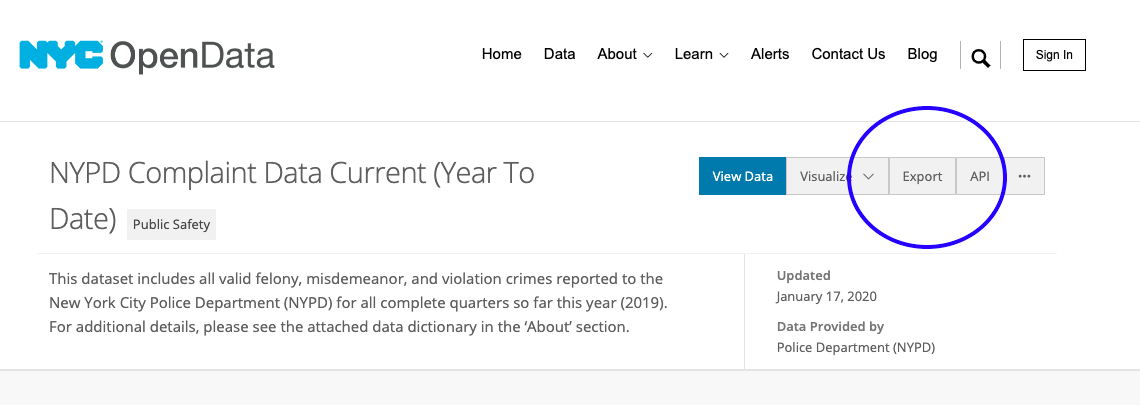
\includegraphics{images/NYPD_CD_main.png}
\caption{Location of Export button on the NYPD Complaint Data page of the NYC open data website}
\end{figure}

If you do this, however, you may end up with a very large file and this may slow things down in terms of download and processing time. For purposes of this first exercise, instead click the View Data button, as this will allow you to filter the data before downloading it:

\begin{figure}
\centering
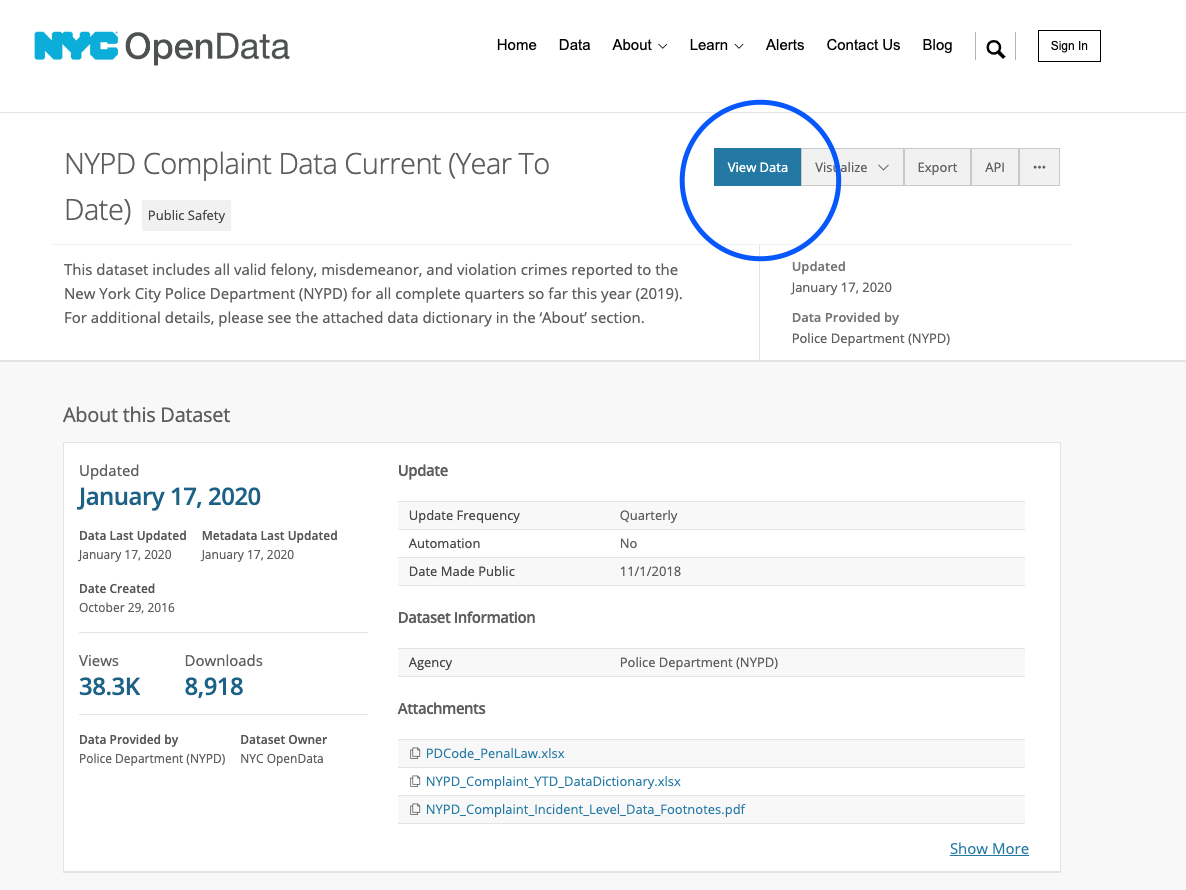
\includegraphics{images/NYPD_CD_view.png}
\caption{Location of the View Data button}
\end{figure}

Clicking on the View Data button will take you to a new page that includes a Filter button. Click on this and then click the Add a New Filter Condition button. You can easily filter the data by any of its fields (or by multiple fields). For this exercise, filter the OFNS\_DESC field (which is the description of the offense, as recorded by the NYPD) for FELONY ASSAULT:

\begin{figure}
\centering
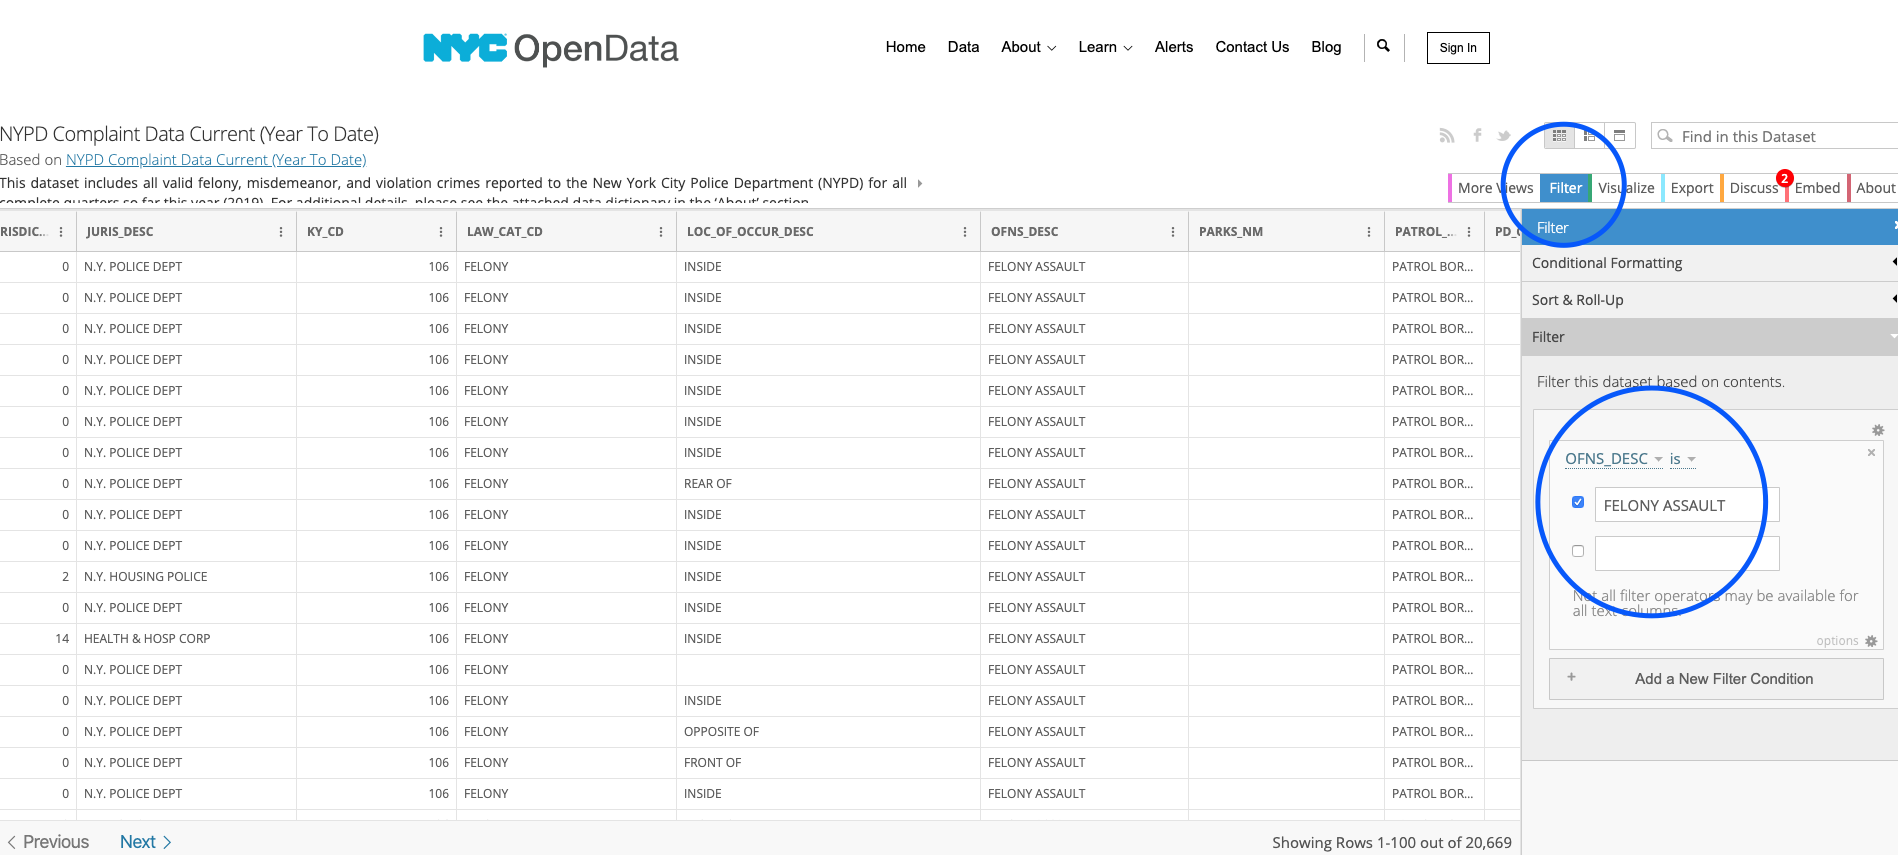
\includegraphics{images/NYPD_CD_filter.png}
\caption{Filtering the NYPD Complaint Data}
\end{figure}

Once you do this, you will see that the effect of the filter in the data displayed in the table on the left, incuding a large reduction in the number of records indicated at the bottom. Now export this filtered data using the Export button and selecting CSV as the format:

\begin{figure}
\centering
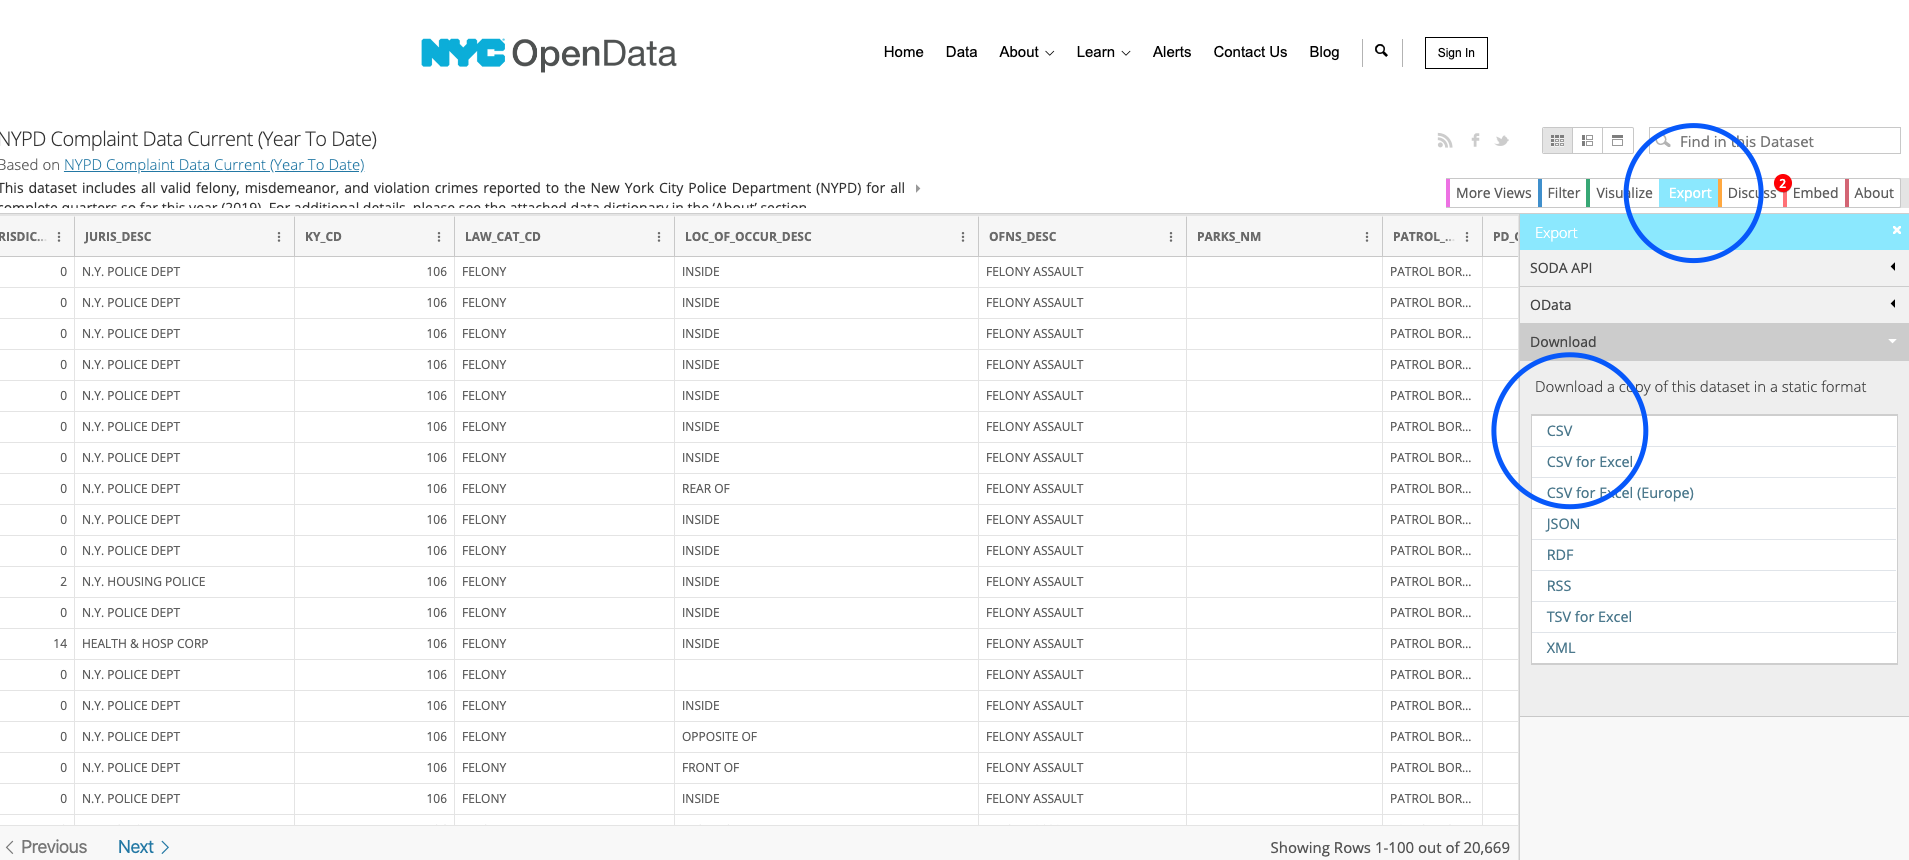
\includegraphics{images/NYPD_CD_visualize_export.png}
\caption{Exporting the NYPD Complaint data}
\end{figure}

Your browser will then let you choose a location to save the downloaded file. Remember this location so that you can find it in the next step and go ahead and complete the download.

\hypertarget{adding-data-to-your-map}{%
\subsection{Adding data to your map}\label{adding-data-to-your-map}}

Add the data to your map using Layer → Add Layer → Add Delimited Text Layer\ldots{}.

\begin{figure}
\centering
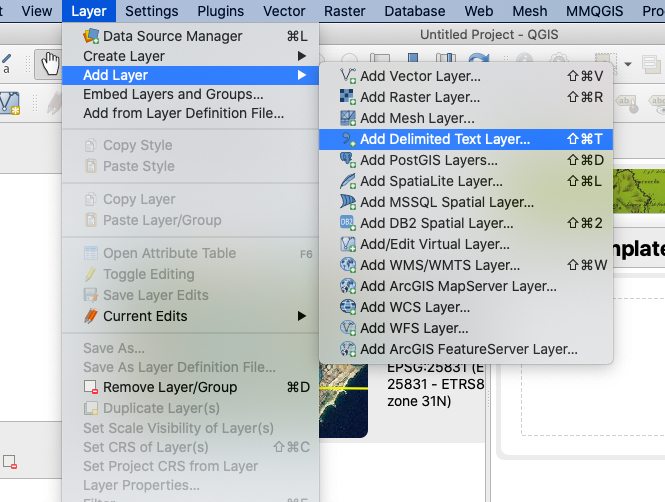
\includegraphics{images/add_deilmited_text_layer.png}
\caption{Screenshot of the Add Delimited Text Layer menu option in QGIS 3.10 for MacOS}
\end{figure}

In the dialog that comes up, click on the \ldots{} button to the right of the File name box at the top. Select the data file you just downloaded and saved.

\begin{figure}
\centering
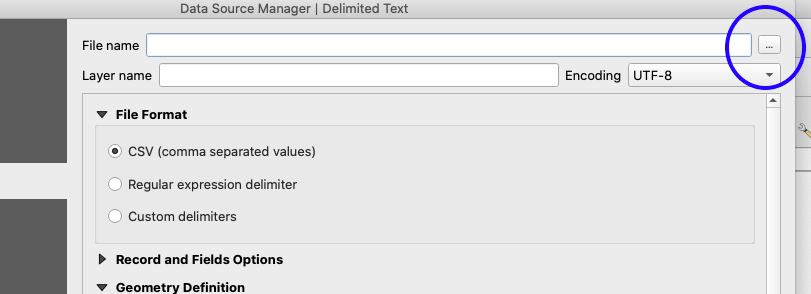
\includegraphics{images/add_delimited_file_chooser.png}
\caption{Choosing file in the dialog (botton at top right with bllue circle around it.)}
\end{figure}

Once you select the file in the dialog box, you will see that it is listed in the File name box. Note that you can also choose a Layer name. This is how the layer you are creating will be named on the layers bar of your QGIS interface. You will need to ensure that the proper File format is selected (in this case CSV) and you will need to provide information about geometry: In the Geometry definition box, make sure Point coordinates is selected. Make sure that the X field and Y field boxes contain the correct field names from your data for the x and y coordinates (in this case, the correct fields are Longitude and Latitute).

Now look at the Coordinate Reference System (CRS) selector, which is labelled Geometry CRS. This is a crucial setting because selecting the wrong CRS will lead to your layer being incorrectly placed on the map (or sometimes not visible at all). For points recorded as Latitude and Longitude, the correct CRS is EPSG 4326 - WGS 84, so make sure this is selected. We will talk more about other CRSs and how to determine which one your data relies on.

Note: Some of these settings may already be correctly set because QGIS automatically tries to figure them out from your file. So in many cases you will simply need to go through and double check them.

Once you have ensured that the settings are correct, look at the preview shown in the Sample Data section at the bottom of the window. You should see a table with data in rows and columns with headers. If you do not see this, go back and check the settings again.

Note: One common problem when importing CSV data is that QGIS may not be properly recognizing the character used to separate columns. CSV stands for comma-separated values, and in many systems this means that the columns are separated with commas (``,'') (as the name implies). In some systems, however, the default is to use semi-colons (``;'') instead of commas - and this is often the default on computers and software localized for Spain. Thus, for example, if you save an Excel sheet as a CSV file on a UPF lab computer, you may find that it is saved using semi-colons rather than commas. You can easily see whether it is commas or semi-colons (or something else) by simply opening your CSV file in a text editor and looking at it closely. If it is not a comma, you will need to specify which character it is by choosing the Custom delimiters setting and then either checking one of the preset boxes or simply typing in the character in the Others box.

Once you have finished with the settings, click the Add button at the bottom of the window.

\hypertarget{adding-data-using-an-api}{%
\subsection{Adding data using an API}\label{adding-data-using-an-api}}

We just added data by first downloading it to your computer because you will often need to work with data files in this way. Data providers, however, are increasingly making it possible to access their data sources using an Application Programming Interface (API). This can simply things for you, particularly when you will be working with a source frequently and will want the most updated data. We will discuss ways of working with APIs later on.

\hypertarget{working-with-multiple-layers}{%
\section{Working with Multiple Layers}\label{working-with-multiple-layers}}

When you first add the NYPD Complaint Data (or any other data source), you should be able to see it in the QGIS mapping window. Often, however, you will want to combine it with additional layers. For example, the NYPD Complaint Data will be much more useful it it is overlaid on top of a map of New York City. You can add such a map in many ways, but for now add Open Steet Map tiles using the instructions in Section \ref{osm-tiles}.

One issue you wil sometimes need to deal with is finding the features in a particular layer you have added. For example, if you have first added Open Street Map tiles and then added points, it may be that your map winder is focused on part of the world where there are no points. To view your new layer, you will need to pan and zoom to get to the location where it actually has data - in this case New York City. You can do that quickly by right-clicking on the layer in the Layers panel and selecting Zoom to Layer at the very top of the menu.

You may also need to make sure that the layer is not being covered by another layer. The order of the layers in the Layers Panel is the order in which they appear on the map (imagine actual layers of paper or transparent paper with features on a physical map). You can drag layers up and down in that list to change the order.

To learn more about each point marked on the map, select View → Identify Features and click on a point. You will see information in the Identify Results panel on the right (although you may need to expand that panel to see the values associated with each feature.

\hypertarget{printing-or-exporting-a-map}{%
\section{Printing or Exporting a Map}\label{printing-or-exporting-a-map}}

What you see in the QGIS console is useful for creating, modifying, and analyzing your map. If you want to share your map with someone or publish it as part of a report, you will want to use the print composer to produce high-quality output.

\hypertarget{setting-up-the-print-layout}{%
\subsection{Setting up the Print Layout}\label{setting-up-the-print-layout}}

Select Project → New Print Layout. In the dialog box that pops up, you can give this print layout a title or leave the box blank and click OK for the default title. You will now see a new window with a canvas that you can use to compose exactly how you want your map to look.

\hypertarget{adding-a-map}{%
\subsection{Adding a map}\label{adding-a-map}}

The most obvious thing you will want on your composed map is the map itself. Select Add Item → Add Map and then use the mouse to draw a rectangle on the canvas where you want the map to appear. Notice that the map that will now appear in that box is essentially a mirror image of the map you currently have in the main console (although the dimensions may be different depending on how you draw the box). After drawing the box, you can still move it around using the Edit → Select/Move Item tool, and you can move the map around within it using the Edit → Move Content tool. Notice that you can add more than one map to your canvas. This makes it possible to include inset maps, for example, showing where your detailed map lies at a larger scale.

\hypertarget{adding-a-scale-bar}{%
\subsection{Adding a scale bar}\label{adding-a-scale-bar}}

You may wish to add a scale bar to your map, and you can do this easily using Add Item → Add Scale Bar. Again, you will need to click on the map to position and resize the scale bar. You will notice that you also have many options to choose from in changing its appearance using the Item properties tab on the right.

\hypertarget{adding-a-legend}{%
\subsection{Adding a legend}\label{adding-a-legend}}

To add a legend, select Add Item → Add Legend and use the mouse to draw a rectangle where you want the legend to appear. The legend will be automatically filled with the information in your layers list, but you can modify this using the Item properties tab on the right. Select the legend you have added and scroll down the Item properties to the Legend Items section. Uncheck Auto update. Now select the layers you do not wish to see in the legend and click the minus sign at the bottom to remove them. Next click the item(s) that you want in the legend and use the editing button to edit the text that will appear. In the Main properties section you can also change the title and alignment of the legend text.

\hypertarget{exporting-your-map}{%
\subsection{Exporting your map}\label{exporting-your-map}}

When you are happy with your map, use Layout → Export as Image or Layout → Export as PDF or Layout → Export as SVG to export your map to a single file, which you can then share, embed in a report, or print.

\hypertarget{vector-from-raster}{%
\chapter{Creating Vector Data From Raster Base}\label{vector-from-raster}}

It will often be necessary to create vector data -- points, lines, or polygons -- by tracing features on an existing raster map. This chapter will walk you through that process.

\hypertarget{obtaining-a-raster}{%
\section{Obtaining a raster}\label{obtaining-a-raster}}

We will start by finding and downloading a raster base For example, you could use a high resolution orthophoto, such as those available at http://www.icc.cat/appdownloads/index.html. When you first enter this site, it will be set to download topographical maps. Change this setting to orthophoto by clicking on the ``Ortoimatges'' tab in the left sidebar. Also change the format option in the bottom of the left sidebar to ``tif'' (for GeoTiff), and select the highest resolution: 1:2.500. Now drag the green square in the mapping area to the region you want to download. For this exercize, zoom in and select UPF's Jaume I building, reducing the size of the green box as you do this so that it just covers the building itself. (Note that with this resolution selecting a large area will result in a very large file.) Once you have the green box in place, click the Descarregar button and enter your email address. The platform will a link to the file to your email within a few moments and you can then click to download it.

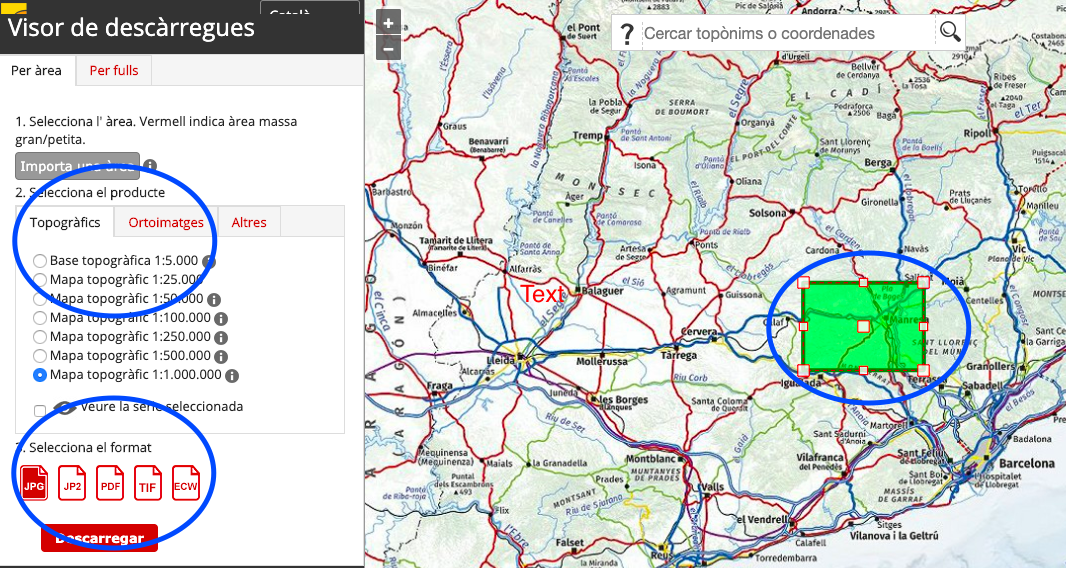
\includegraphics{images/icc_map.png}
\#\# Adding raster to map

By saving the file in GeoTiff format you have ensured that it includes CRS information that QGIS can read automatically. Add the layer using Layer → Add Layer → Add Raster Layer\ldots{} and then selecting the file you downloaded. Depending on the CRS of your current map, QGIS may then give you a choice of how to transform your raster's CRS to the map's CRS. You can select one of these or you can go back to your map and change it's CRS to match the raster's.

\begin{figure}
\centering
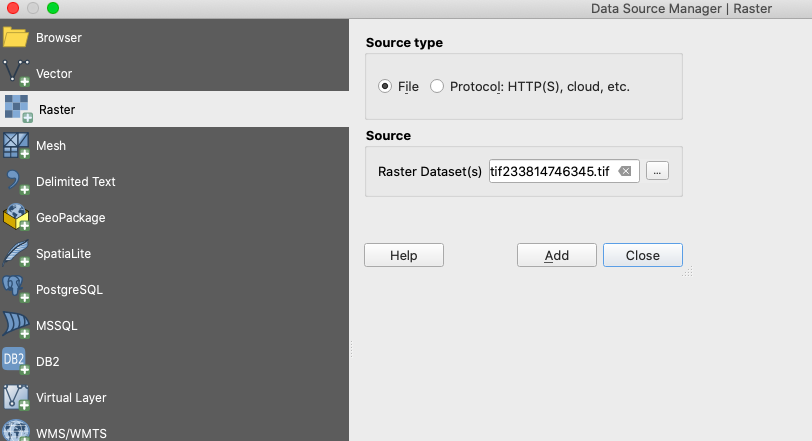
\includegraphics{images/adding_raster_layer.png}
\caption{Adding raster layer.)}
\end{figure}

\hypertarget{creating-a-new-vector-layer.}{%
\section{Creating a new vector layer.}\label{creating-a-new-vector-layer.}}

Create a new vector layer using Layer → Create Layer → New Shapefile Layer\ldots{}. In the window that pops up, you can choose to make this a layer of points, lines, or polygons (see Geometry Type selector, third from top). You can also modify the character encoding (File Encoding selector), the CRS (selector just below the File Encoding selector), and the data fields that will be associated with this new layer.
For this exercise, choose Polygon as the type, and add at least one new field in which you will store information associated with each feature that you draw. For this exercise, we will be using the layer to indicate the approximate number of people who you observed in the courtyard during our first lab, so create a Whole Number field and give it a name (e.g.~N). Save the new layer as an SHP file in a directory where you will be able to find it again.\\
\#\# Adding features

The new layer you have added should appear in the Layers Panel. Right click on this new layer and select Toggle Editing. You will now see a set of new buttons and available menu items. Select Edit → Add Polygon Feature. When you hover the mouse pointer over the map you will see that it now has the shape of a cross-hairs. Left click to add sequential points that define the polygon you want to add. When you have added the last point, right click the mouse and a dialog box will appear asking you to add the fields associated with this new feature. Remember that what you add will be limited by the field type you chose (and the ID field requires whole numbers by default). For this exercise, draw a rectangle over UPF's Jaume I courtyard.

\hypertarget{vector-appearance}{%
\chapter{Adjusting Vector Layer Appearance}\label{vector-appearance}}

QGIS gives you control over how your vector layers appear: You can adjust color, fill style, transparency, labeling, and many other characteristics.

\hypertarget{opening-the-properties-window}{%
\section{Opening the properties window}\label{opening-the-properties-window}}

To do this, you need to start by opening the Layer Properties window. Right click on the layer you want to adjust and select Properties. You will see a new window with a set of tabs on the left.

\hypertarget{changing-fill-color-border-and-style}{%
\section{Changing fill color, border and style}\label{changing-fill-color-border-and-style}}

To change the layer's color, select the Symbology tab. If this is a polygon layer, you will see a box with Fill and under this Simple fill. Click on Simple fill and then scroll down adn click the Fill color selector and choose a color. Notice that you have different options for picking the color, including choosing one from a pallet or gradient, entering HSV or RGB values, or entering an HTML code. You can also choose the level of opacity, which lets you make semitransparent features. (Note that this can be set for the fill color itself or for the entire layer.)

You can also change the border and fill style using the Stroke color and Fill style selectors.

\hypertarget{adding-labels}{%
\section{Adding labels}\label{adding-labels}}

To add labels to your layer, select the Labels tab. At the very top of the window, change the selector from No labels to Single labels. Just underneath this selector, you will see a selector for Value. Use this to select the field you wish to use for your labels. If you created a field in the exercise above for number of people, you can use this to automatically display this information on each feature. Alternatively, you might have a field for name or ID. The idea here is that QGIS can automatically use one of the fields to generate labels. Try making labels and click OK to see how they look. Then return to the Properties window to explore the various options you have for adjusting the labels' appearance.

\hypertarget{osm-vectors}{%
\chapter{Adding OpenStreetMap vectors}\label{osm-vectors}}

One useful way to add existing vector information to a map, while also making it possible to customize its appearance, is to download data from OpenStreetMap (OSM). The process will be to download the OSM file for a given area, then open it, choose the layers that you want, filter these layers according to feature type, and then modify appearances. To do this, you will need to install the OSMDownloader plugin. Open the Plugins menu, choose Manage and Install Plugins\ldots{}. Search for ``OSMDownloader'' and install it. Notice that a small button now appears on the top left, just above the left pane. This is what you will use for downloading the vector data.

\hypertarget{downloading-osm-data}{%
\section{Downloading OSM data}\label{downloading-osm-data}}

Start with some raster base map that lets you navigate to a place of interest (OSM map tiles, an orthophoto etc.). Zoom in to a small area (if the area is too large, the download size can be huge). For purposes of this exercise, zoom to the area immediately around UPF's Ciutadella campus (no more than a few blocks). Now click the OSMDownload button at the top left and drage the cursor on the map to select the rectangle for which you will download vector data.

\begin{figure}
\centering
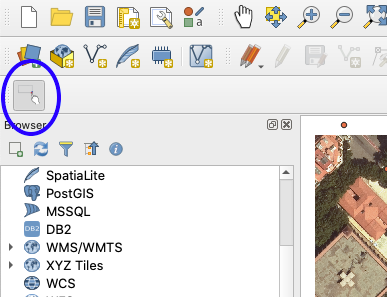
\includegraphics{images/osmdownloader_button.png}
\caption{Adding raster layer.)}
\end{figure}

In the window that appears, select Save File and choose a name and directory for the files you will download. Also click the Load Layer After Download box. Then click OK. Once the data is downloaded, you will see a new window with a list of layers that this file contains. You can select some or all of these. When you hit OK you will see each of these layers appear on your map and in your Layers Panel.

\hypertarget{labeling-the-vector-data}{%
\section{Labeling the vector data}\label{labeling-the-vector-data}}

You can add labels to this new layer just as you did above. You may find, however, that there is too much information and that you want to filter it somehow. You can filter the labels themselves using the labels tab. Or you can filter the features in the layer as follows.

\hypertarget{filtering-the-vector-data}{%
\section{Filtering the vector data}\label{filtering-the-vector-data}}

To filter a layer, right click on it and it and choose Filter. This will bring up a new window in which you can write a query to filter the features in this layer according to their attribute fields. To do this, you need to know something about what these fields contain, and you can see this by clicking on a field and hitting the Sample button. You can then create a filter by double clicking on a field name, clicking an operator, and then double clicking a value. You will see the query being built as you do this in the box at the bottom. For example ``highway''=`tertiary' would filter the features to include only those for which the ``highway'' field has the value (character string in this case) `tertiary'.

Another way of filtering, which is often easier, is to start by coloring the features according to some field of interest. Open the Properties window for the layer. In the Symbology tab, select Categorized in the selector at the top. Then choose the field you want to use for this in the Value selector. Hit the Classify button and QGIS will assign a different random color to each different value that appears in this field. Click OK to see how this looks on the map. You can now click the field in the Layers Panel to expand it to show each unique value and the color assigned to it. You can click any of these to remove or return it to the map.

\hypertarget{aggregated-data}{%
\chapter{Mapping Aggregated Data}\label{aggregated-data}}

\hypertarget{choropleth-maps}{%
\section{Choropleth Maps}\label{choropleth-maps}}

\hypertarget{downloading-data-1}{%
\subsection{Downloading data}\label{downloading-data-1}}

For this exercise, we will use 2013 data extracted from the Eurostat database Recorded offences by offence category - police data. You can download it directly from that site, but to make things easier I have already done some data cleaning and you can download the cleaned data here:

Download Data

\hypertarget{download-and-unzip-shapefiles}{%
\subsection{Download and Unzip Shapefiles}\label{download-and-unzip-shapefiles}}

We will map this data using the Eurostat Countries 2013 shapefiles at the 1:3 million scale. Download them here:

Download Shapefiles

The file you have downloaded is a zipped archive of shapefiles. Find the directory in which you saved it and double click on the file to unzip it.

\hypertarget{add-country-boundaries-to-map}{%
\subsection{Add Country Boundaries to Map}\label{add-country-boundaries-to-map}}

Add the country boundaries using Layer → Add Layer → Add Vector Layer.

In the Data Source Manager window that pops up, leave Source type as it is (the default is File with System encoding), and click the button in the Source section to select the shapefiles you want to add. Navigate to the directory in which you unzipped these files look at what you have. You will see a number of sets of files with identical names. Each set represents a different layer. We will be using CNTR\_RG\_03M\_2013, but go ahead and add all of them just to see what they look like. To do this, sort the files by type and then hold down the Shift key will clicking on all of the files that have the .shp extension. (QGIS will automatically open all associated files, which have the same names but different extensions).

After selecting the files, click ``Open'' in the two dialog windows, and the shapes should appear on the map. (Remember that the order of the layers in the layer panel controls the order on the map and that you may need to change this to view certain layers.)

\hypertarget{adding-the-data}{%
\subsection{Adding the data}\label{adding-the-data}}

Add the data using Layer → Add Layer → Add Delimited Text Layer\ldots{}.

In the File Name box, select the data file (for this exercise, it is crim\_off\_cat\_rates.csv if you did not change the name when saving it). In the File format box, choose CSV if it is not already chosen. Look in the preview area below and see if the data is appearing in an organized way, with column headings and values. (It should be for this exercise, but if you use a different data set in the future and it is not appearing correctly, the first thing to try is selecting the Custom delimiters option for File format and trying the Semicolon option or something else.) For Geometry definition, select No geometry (attribute only table). This data source does not have coordinates. It simply has data by country name and you will need to link those country names to your shapes in the following step. Click OK.

\hypertarget{join-the-country-polygons-with-the-data.}{%
\subsection{Join the country polygons with the data.}\label{join-the-country-polygons-with-the-data.}}

In the layers panel, right click on the country boundary layer (which will be called CNTR\_RG\_03M\_2013 if you have not changed the names) and select Properties. In the properties window, select the Joins tab.

To join the data to the polygons, there needs to be a field in the data table that contains a set of unique identifiers corresponding to a set of the same unique identifiers in the polygon attribute table. For this exercise, the GEO field in the data table has country codes that correspond to the same country codes in the polygon attribute table's CNTR\_ID field. (When you are using your own data sources, this will often require some initial cleaning. For example, you may need to convert country codes to make sure they match, or you may need to deal with complications like states, like Yugoslavia, that have broken apart or those, like Germany, that have formed through unification.)

Click the plus button at the bottom left. For Join layer, select your data you want to join (for this exercise it is crim\_off\_cat\_rates). For Join field, select the field in the data table that you will be using for this join. In this case, GEO. For the Target field, select the field in the polygon attribute table that you will be using for the join. In this case, CNTR\_ID). Click OK and then Apply.

\hypertarget{color-the-polygons-according-to-crime-data}{%
\subsection{Color the polygons according to crime data}\label{color-the-polygons-according-to-crime-data}}

In the Style panel, choose Graduated in the selector at the very top. Now select for Column the field you want to represent on the map. Since you have joined the data with this polygon layer, you will be able to choose from the fields in the data table as well as in your polygon attribute table. For this exercise, choose crim\_off\_cat\_rates\_Theft). Select a Color ramp that you like. Under the Classes tab, select a choice for Mode. You can experiment with different options and see how they appear. Now click the Classify button and then click OK.

\hypertarget{clean-the-map}{%
\subsection{Clean the map}\label{clean-the-map}}

Use the layers panel to remove any unnecessary layers that are distracting (for instance, if you included all of the shape files in the Eurostat country data). Use the zoom and pan tools to focus the map on the area of interest to you.

\hypertarget{proportional-symbols}{%
\section{Proportional Symbols}\label{proportional-symbols}}

The choropleth map you just produced represents quantitative data using colors. But it is limited to showing one field from your data. What if you want to show additional information? One option would be to add a symbol on top of each color, making the size proportional to the additional values you want to display. In other words, one field will be displayed by color and another by size.

If you added all of the shapefiles that you downloaded in the last exercise, then you already have everything you need. Put a check next to the CNTR\_LB\_2013 layer in your layers panel to display a point for each country on top of the choropleth. You will use these points to place your proportional symbols. Right-click on this layer and select Properties. Use the same approach as in the last exercise to join this layer to your data table.

\hypertarget{style-the-point-symbols-using-graduated-sizes}{%
\subsection{Style the point symbols using graduated sizes}\label{style-the-point-symbols-using-graduated-sizes}}

In the Style panel, select Graduated at the top and choose the Column you want to represent here. For this exercise, choose crim\_off\_cat\_rates\_TOTAL. For Method now select Size. Choose a Mode and click Classify. You will need to play around with classification modes as well as minimum and maximum sizes to create symbols that are useful for explaining your data. Click OK to display the result on your map.

\hypertarget{pie-charts}{%
\section{Pie Charts}\label{pie-charts}}

To include even more information on your map, you may want to include some small charts that are then placed on top of geographic features. for this exercise we will use pie charts.

Return to your point layer properties and now select the Diagrams tab. At the top, select Pie chart. For attributes, select all of the individual crime categories that you want to include. Be careful not to include overlapping information here. Use the plus button to move all of these to the Assigned attributes list. You can also size your pie charts proportionally to another variable using the size tab here.

\hypertarget{aggregating-point-data}{%
\chapter{Aggregating Point Data}\label{aggregating-point-data}}

\hypertarget{counting-points-in-areal-units}{%
\section{Counting Points in Areal Units}\label{counting-points-in-areal-units}}

\hypertarget{obtain-the-data}{%
\subsection{Obtain the data}\label{obtain-the-data}}

For this exercise, we will again use the New York City assault data extracted from NYC Open Data, which you can download by clicking the button below.

Download the data

\hypertarget{obtaining-shapefile}{%
\subsection{Obtaining shapefile}\label{obtaining-shapefile}}

We will use the polygons in the New York City police precinct geojson shapefile from the same site. You can download it using the button below. If the geojson text appears in a new browser window rather than automatically triggering a download prompt, simply choose Save Page As\ldots{} or else copy the text and past it into a new text file, saving with the geojson extension.

Download geojson shapefile

\hypertarget{add-the-shapefile-layer-to-your-map}{%
\subsection{Add the shapefile layer to your map}\label{add-the-shapefile-layer-to-your-map}}

Add the shapefile to your map with Layer → Add Layer → Add Vector Layer\ldots{}, or with the {} button.

Select the geojson file and click Open.

\hypertarget{add-the-data}{%
\subsection{Add the data}\label{add-the-data}}

Add the data using Layer → Add Layer → Add Delimited Text Layer\ldots{}, or the {} button.

Select the data file (for this exercise it is NYPD\_Complaint\_Map\_\_Year\_to\_Date.csv). On the Geometry definition line, make sure Point coordinates is selected and make sure the Longitude and Latitude fields are selected for the X field and Y field, respectively. Click OK.

In the Coordinate Reference System window that should now pop up, select the appropriate coordinate reference system. If the points are defined by Latitude and Longitude (as in our exercise data), then this should be WGS 84 (EPSG 4326). (If you are using data in another coordinate reference system, make sure you check which this is in the data documentation.)

\hypertarget{count-the-points-in-each-polygon}{%
\subsection{Count the points in each polygon}\label{count-the-points-in-each-polygon}}

To count how many points (crime report locations) fall within each polygon (police precinct), use Vector → Analysis Tools → Count points in polygon.

In the parameters tab of the window that pops up make sure that the correct layers are selected for the polygons and the points, and click Run.

You will now see that a new layer has appeared on your map and inyour layers window. The new layer contains the polygons from your original polygon layer, but it also has an attribute table that links each of these polygons to the count of points that falls within it. The polygons will appear by default with one single fill color, but you can change the style to color them according the count. (For example, follow the \protect\hyperlink{mapping-aggregated-data}{Mapping Aggregated Data} recipes.)

\hypertarget{geocoding}{%
\chapter{Geocoding}\label{geocoding}}

Geocoding is the process of converting addresses into geographic coordinates. We can do this in QGIS using the MMQGIS Plugin.

\hypertarget{install-mmqgis}{%
\section{Install MMQGIS}\label{install-mmqgis}}

Install the MQGIS plugin using Plugins → Manage and Install Plugins and searching for mmqgis.

\hypertarget{obtain-csv-address-file}{%
\section{Obtain CSV address file}\label{obtain-csv-address-file}}

The addresses you want to geocode using MMQGIS need to be in a CSV file that includes fields for address, city, state (province), and country. You could create a file like this using Excel or you may have a file like this already from whatever data source you are working with. For this exercise, use the file here:

Download the address data

\hypertarget{use-the-mmqgis-geocoding-function}{%
\section{Use the MMQGIS geocoding function}\label{use-the-mmqgis-geocoding-function}}

To geocode these addresses, click MMQGIS → Geocode → Geocode CSV with Google / Open Street Map.

In the dialog window that pops up, choose the CSV file with your addresses and make sure the Address, City, State, and Country fields are selected correctly. If you choose to geocode with Google Maps, you may need to obtain an Google API key to avoid limits. The simpler alternative is to use the OpenStreetMap / Nominatum option. You will also need to specify file names for the output file (where the geolocations will be stored) as well as for a file that will store a list of addresses that could not be geocoded. This second part is important because you will need to find ways to locate these addresses (often by modifying the address text). When you have all of this specified, click OK.

If some or all of the addresses could be geocoded, you will see a new points layer appear on your map, containing the locations. Make sure to check the file of addresses that could not be geocoded as well, and figure out what went wrong with these. One common error is with the character encoding. Your csv file needs to be encoded as UTF-8.

\bibliography{book.bib,packages.bib}


\end{document}
